\section{Thiết kế giao diện hệ thống}
\subsection{Giao diện đăng nhập}
\begin{center}
	\includegraphics[width=4cm]{Images/login} \\ 
	Giao diện đăng nhập
\end{center}
$\indent$
Đây là trang đầu tiên khi người dùng mở ứng dụng. Các tài khoản người dùng đều phải được admin cung cấp. Ở trang này, người dùng nhập username và password để đăng nhập vào hệ thống. Đăng nhập thành công sẽ chuyển đến trang chủ. Đăng nhập không thành công thì trang đăng nhập refresh lại.
\subsection{Giao diện trang chủ}
\begin{center}
	\includegraphics[width=4cm]{Images/homepage} \\ 
	Giao diện trang chủ
\end{center}
$\indent$
Đây là trang hiển thị sau khi đăng nhập thành công. Trang hiển thị nhiệt độ, độ ẩm của tòa nhà.
Nhấn vào "Chi tiết", ứng dụng sẽ chuyển sang trang danh sách nhiệt độ, độ ẩm các phòng. 
\subsection{Giao diện danh sách các phòng}
\begin{center}
	\includegraphics[width=5cm]{Images/index } \\ 
	Giao diện danh sách các phòng
\end{center}
$\indent$
Đây là trang hiển thị sau khi nhấn vào nút "Chi tiết" ở trang chủ. Danh sách hiển thị số phòng, nhiệt độ, độ ẩm của từng phòng. Nhấn vào từng phòng thì sẽ hiển thị danh sách thiết bị của từng phòng
\subsection{Giao diện thiết bị trong phòng}
$\indent$
Trang hiển thị số phòng, nhiệt độ, độ ẩm trong phòng, có thể tìm kiếm thiết bị trong phòng.
Ở đây người dùng có thể chọn 2 chế độ Automode hoặc tự mình điều khiển thiết bị.
\subsubsection{Giao diện thiết bị trong phòng với chế độ Automode}
\begin{center}
	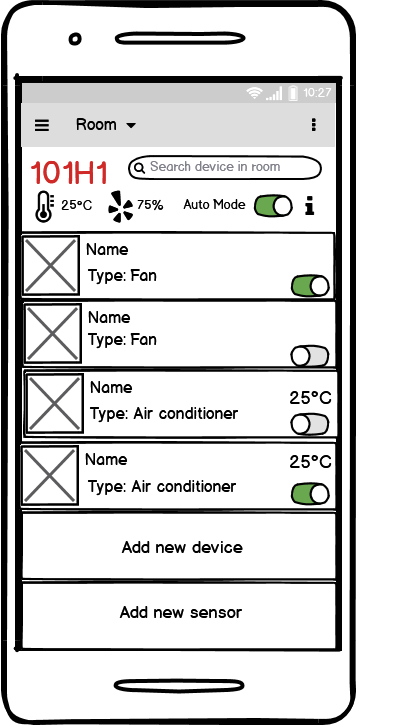
\includegraphics[width=4cm]{Images/Listdeviceautomode.png} \\ 
	Giao diện thiết bị trong phòng ở chế độ Automode
\end{center}
$\indent$Chế độ Automode đang được kích hoạt. Tất cả thiết bị được hiển thị ở đây có thông tin là tên thiết bị, loại thiết bị. Nếu là quạt thì hiển thị trạng thái bật tắt. Nếu là máy lạnh thì hiển thị trạng thái bật tắt và nhiệt độ máy lạnh. \\
$\indent$Người dùng không thể tắt mở, điều khiển thiết bị ở chế độ này. Mọi điều khiển đều được lập trình sẵn. \\
\subsubsection{Giao diện thiết bị trong phòng với chế độ tự điều khiển}
\begin{center}
	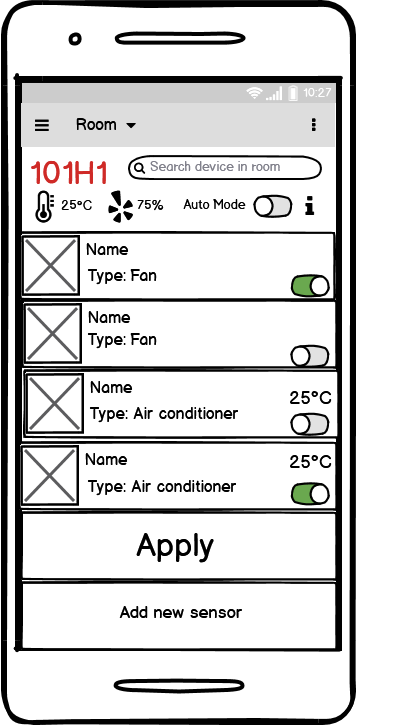
\includegraphics[width=4cm]{Images/Listdevice_user} \\ 
	Giao diện thiết bị trong phòng
\end{center}
$\indent$
Chế độ Automode đã được tắt. Người dùng có thể điều khiển thiết bị ở đây. Sau khi điều chỉnh, người dùng ấn "Apply" để áp dụng những điều chỉnh ở trên.\\
$\indent$Nút "Add new sensor" chỉ hiển thị khi sử dụng tài khoản admin.\\ 
\subsection{Thanh menu}
\subsubsection{Thanh menu của Admin}
\begin{center}
	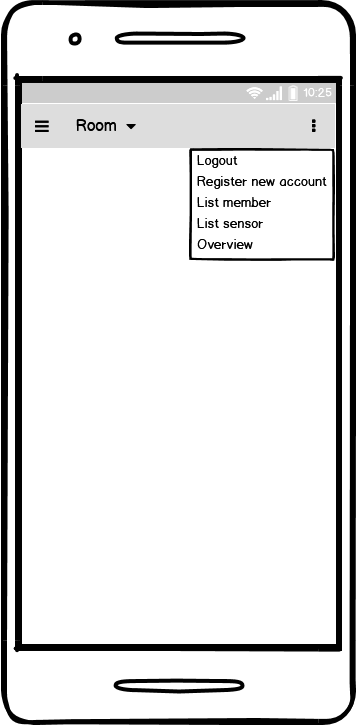
\includegraphics[width=4cm]{Images/Menu Admin} \\ 
	Thanh menu của admin
\end{center}
$\indent$
"Logout": Thoát tài khoản admin. Sau khi thoát, ứng dụng chuyển về trang đăng nhập ban đầu. \\
$\indent$
"Register new account": Thêm tài khoản mới. Sau khi ấn, chuyển đến trang đăng kí tài khoản. \\
$\indent$
"List member": Hiển thị danh sách thành viên trong ứng dụng. \\
$\indent$
"List sensor": Hiển thị danh sách cảm biến trong hệ thống. \\
$\indent$
"Overview": Hiện thị trang phân tích đánh giá của hệ thống. \\
\subsubsection{Thanh menu của User}
\begin{center}
	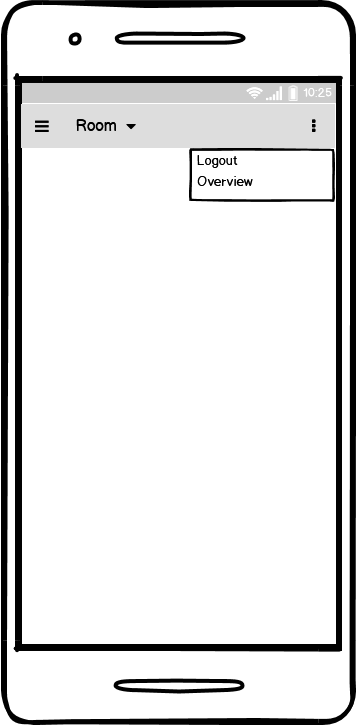
\includegraphics[width=4cm]{Images/Menu User} \\ 
	Thanh menu của user
\end{center}
$\indent$
"Logout": Thoát tài khoản admin. Sau khi thoát, ứng dụng chuyển về trang đăng nhập ban đầu. \\
$\indent$
"Overview": Hiện thị trang phân tích đánh giá của hệ thống. \\
\subsection{Giao diện đăng ký tài khoản}
\begin{center}
	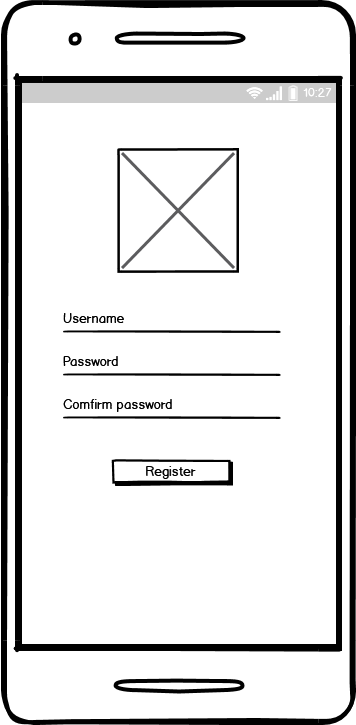
\includegraphics[width=4cm]{Images/Register} \\ 
	Giao diện đăng kí tài khoản mới
\end{center}
$\indent$
Admin tạo tài khoản mới cho người dùng. Nếu tài khoản hợp lệ (username không trùng với những username cũ, mật khẩu dài hơn 8 kí tự) thì hiển thị thông báo "Tạo tài khoản thành công!".
\subsection{Giao diện phân tích, đánh giá tổng quan}
\begin{center}
	\includegraphics[width=4cm]{Images/Overview } \\ 
	Giao diện phân tích, đánh giá tổng quan
\end{center}
$\indent$
Giao diện hiển thị nhiệt độ, độ ẩm của từng ngày, tháng,... \\
\subsection{Giao diện danh sách cảm biến}
\begin{center}
	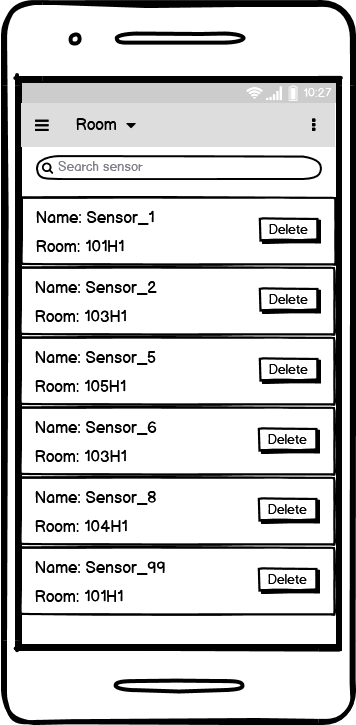
\includegraphics[width=4cm]{Images/ListSensor} \\ 
	Giao diện danh sách cảm biến
\end{center}
$\indent$
Giao diện chỉ có admin mới xem được. Admin có thể xóa sensor đó ra khỏi danh sách sensor của ứng dụng. \\
\subsection{Giao diện danh sách cảm biến mới}
\begin{center}
	\includegraphics[width=4cm]{Images/Add Sensor} \\ 
	Giao diện danh sách cảm biến mới
\end{center}
$\indent$
Sau khi ấn "Add new sensor", ứng dụng sẽ hiển thị danh sách cảm biến mới mà ứng dụng chưa thêm vào. Ấn "Add" để thêm cảm biến mới vào.
\subsection{Giao diện danh sách thành viên}
\begin{center}
	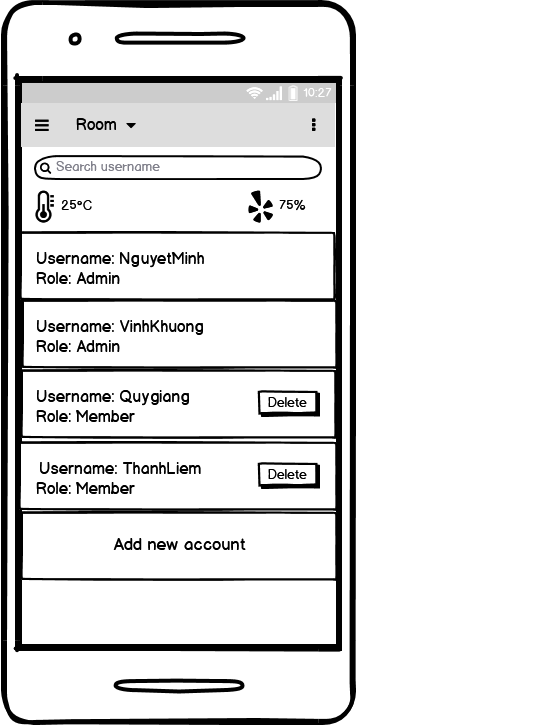
\includegraphics[width=5cm]{Images/List member} \\ 
	Giao diện danh sách thành viên
\end{center}
$\indent$
Giao diện này chỉ có admin mới xem được. Admin được quyền xóa tài khoản của Member nhưng không được xóa tài khoản các admin khác. \\
\section{Thiết kế cơ sở dữ liệu}
\subsection{ERD}
\begin{center}
	\includegraphics[width=\columnwidth]{Images/EERD} \\ 
\end{center}
\subsection{RMapping}
\begin{center}
	\includegraphics[width=\columnwidth]{Images/MappingFinal} \\ 
\end{center}
\section{Báo cáo giải thuật, công nghệ tìm được}
$\indent$\textbf{Tính toán số lượng thiết bị}\\
$\indent$•	Tổng cảm biến 1 phòng = tổng số cảm biến nhiệt độ + tổng số cảm biến độ ẩm phòng đó\\
$\indent$•	Tổng thiết bị 1 phòng =  tổng số quạt + tổng số máy điều hoà phòng đó\\
$\indent$•	Tổng cảm biến cả toà = tổng cảm biến các phòng có trong toà\\
$\indent$•	Tổng thiết bị các toà = tổng thiết bị các phòng có trong toà\\

\textbf{Các công thức tính trung bình:}\\
$\indent$•	Nhiệt độ trung bình của một phòng = Tổng nhiệt độ các cảm biến nhiệt độ trong phòng : tổng số cảm biến nhiệt độ phòng đó\\
$\indent$•	Độ ẩm trung bình của một phòng = Tổng độ ẩm các cảm biến độ ẩm trong phòng : tổng số cảm biến độ ẩm phòng đó\\
$\indent$•	Nhiệt độ trung bình ngày của cả toà  = Tổng nhiệt độ trung bình của cả toà đo các lần trong ngày : số lần đo.\\
$\indent$•	Độ ẩm trung bình ngày của cả toà = Tổng giá trị độ ẩm trung bình của cả toà đo các lần trong ngày : số lần đo.\\

Gọi t là giá trị nhiệt độ nhận được, h là giá trị độ ẩm nhận được.\\
\textbf{$\indent$Hiển thị đánh giá tổng quát\\}
$\indent$Phân loại nhiệt độ theo thang, gọi t là giá trị nhiệt độ nhận được\\
$\indent$•	$20^{o}C$  < T <= $25^{o}C$: khí hậu mát mẻ\\
$\indent$•	$25^{o}C$ < T <= $30^{o}C$: nhiệt độ bình thường\\
$\indent$•	$30^{o}C$ < T <= $33^{o}C$: thời tiết oi bức, nên bật điều hoà và quạt\\
$\indent$•	T > $33^{o}C$:   cảnh báo nguy cơ cháy nổ, thiếu nước, nên bật điều hoà và quạt\\

\textbf{Phân loại độ ẩm theo thang\\}
$\indent$•	H <= 30\% : cảnh báo độ ẩm cực kỳ thấp, nguy cơ cháy nổ cao.\\
$\indent$•	30\% < H <= 50\%  : độ ẩm thấp, đề phòng thiếu nước, nứt nẻ chân tay, môi,...\\
$\indent$•	50\% < H <= 60\%  : độ ẩm mức giao thoa, vẫn đạt ngưỡng cho phép.\\
$\indent$•	60\% < H <= 80\% : độ ẩm phù hợp với môi trường, khí hậu con người.\\
$\indent$•	80\% < H <= 90\%  : khí hậu thay đổi, đề phòng nguy cơ cảm cúm, ốm, sốt\\
$\indent$•	H > 90\%             : độ ẩm cao,  đề phòng nguy cơ cảm cúm, ốm, sốt, chú ý bảo trì các vật dụng đề phòng nấm mốc, hỏng hóc

\textbf{Thang bật tắt các thiết bị tự động}\\
$\indent$•	Quạt: \\
$\indent$Khi T > $30^{o}C$, quạt tự động được bật\\
$\indent$Khi T <=  $25^{o}C$, quạt tự động được tắt\\
$\indent$•	Điều hoà:\\
$\indent$Khi T > $30^{o}C$ và H > 60\%: bật điều hoà ở chế độ dry và nhiệt độ T - $6^{o}C$.\\
$\indent$Khi T > $30^{o}C$ và H < 60\%: bật điều hoà ở chế độ cool và nhiệt độ t - $6^{o}C$.\\
$\indent$Khi T < $20^{o}C$ và H < 60\%: bật điều hoà ở chế độ cool và nhiệt độ t + $6^{o}C$.\\
$\indent$Khi T < $20^{o}C$ và H > 60\%: bật điều hoà ở chế độ dry và nhiệt độ t + $6^{o}C$.\\
$\indent$Khi $20^{o}C$ <= T <= $25^{o}C$ : điều hoà tự động tắt.\\
\section{Bảng phân công nhiệm vụ}
\begin{center}
	\begin{tabular}{ | m{4cm} | m{10cm}|  } 
		\hline
		\textbf{Họ và tên}&\textbf{Phân công công việc  } \\ 
		\hline
		Ngô Thanh Liêm & - Vẽ ERRD\\ 
		\hline
		Cao Nguyệt Minh & - Thiết kế giao diện hệ thống, viết báo cáo\\
		\hline
		Đinh Vĩnh Khương & - Thiết kế giao diện trang chủ, viết báo cáo giải thuật \\
		\hline
		Võ Quý Giang & - Vẽ R-Mapping\\
		\hline
	\end{tabular}
\end{center}
\section{Tài liệu tham khảo}
\begin{enumerate}
\item https://vcs.vn/bang-thang-do-do-am-khong-khi-tai-lieu-vcs-vn
\item https://www.dienmayxanh.com/kinh-nghiem-hay/nen-de-dieu-hoa-o-che-do-cool-hay-dry-che-do-nao-t-1128235
\end{enumerate}
\end{document}



